\documentclass[a4paper]{article}
\usepackage[margin=2cm,includeheadfoot,
nomarginpar,]{geometry}

%\usepackage{luacode}
\usepackage{listings, listings-rust}

\usepackage{authblk}
\usepackage{color, xcolor}
\usepackage{tikz}
\usetikzlibrary{shapes, shadows}



\usepackage{lipsum} % Dummy text for demonstration

% Bibliography
\usepackage[style=apa, parentracker=true]{biblatex}
\addbibresource{myLibrary.bib}


% Code Snippets Styling
\renewcommand\lstlistingname{Source Code}
\renewcommand\lstlistlistingname{Source Code}

\definecolor{codebg}{rgb}{0.11,0.12,0.13} % Dark background
\definecolor{codebasic}{rgb}{0.73,0.74,0.76} % Dark background
\definecolor{codecomment}{rgb}{0.44,0.45,0.47} % Gray for comments
\definecolor{codestring}{rgb}{0.41,0.60,0.31} % Green for strings
\definecolor{codekey1}{rgb}{0.97,0.33,0.39} % Red for keywords
\definecolor{codekey2}{rgb}{0.20,0.13,0.79} % Red for keywords

\lstdefinestyle{mystyle}{
	language=Rust, 
	backgroundcolor=\color{codebg},
	basicstyle=\ttfamily\footnotesize\color{codebasic},
	commentstyle=\color{codecomment}, 
	stringstyle=\color{codestring},
	keywordstyle=\bfseries,% reserved keywords
	%keywordstyle=[2]\color{codekey2},% traits
	%keywordstyle=[3]\color{codekey2},% primitive types
	%keywordstyle=[4]\color{codekey2},% type and value constructors
	keywordstyle=[5]\color{codekey1},% macros
	%
	breaklines=true,
	breakatwhitespace=true, 
	numbers=left,
	firstnumber=auto,
	numbersep=5pt,
	tabsize=4,
	xleftmargin=10pt,
	showstringspaces=false,
	showspaces=false,
	showtabs=false,
	columns=spaceflexible,
	keepspaces=true,
	frame=left,
	framesep=5pt,
	framerule=10pt,
	rulecolor=\color[gray]{0.30},
	mathescape=true,
	captionpos=b,
}





% Document Info
\title{\LaTeX\ Template}
\author[1]{Marco Ramos}
\affil[1]{Coventry University, Coventry, UK}


\begin{document}
	% COVER PAGE
	\newgeometry{margin=0pt} % Set zero margins for the first page
\thispagestyle{empty} % Remove page number and header/footer for the first page


\hspace*{-0.61cm} %shift left
\vspace*{-1cm} %allow negative y coordinates
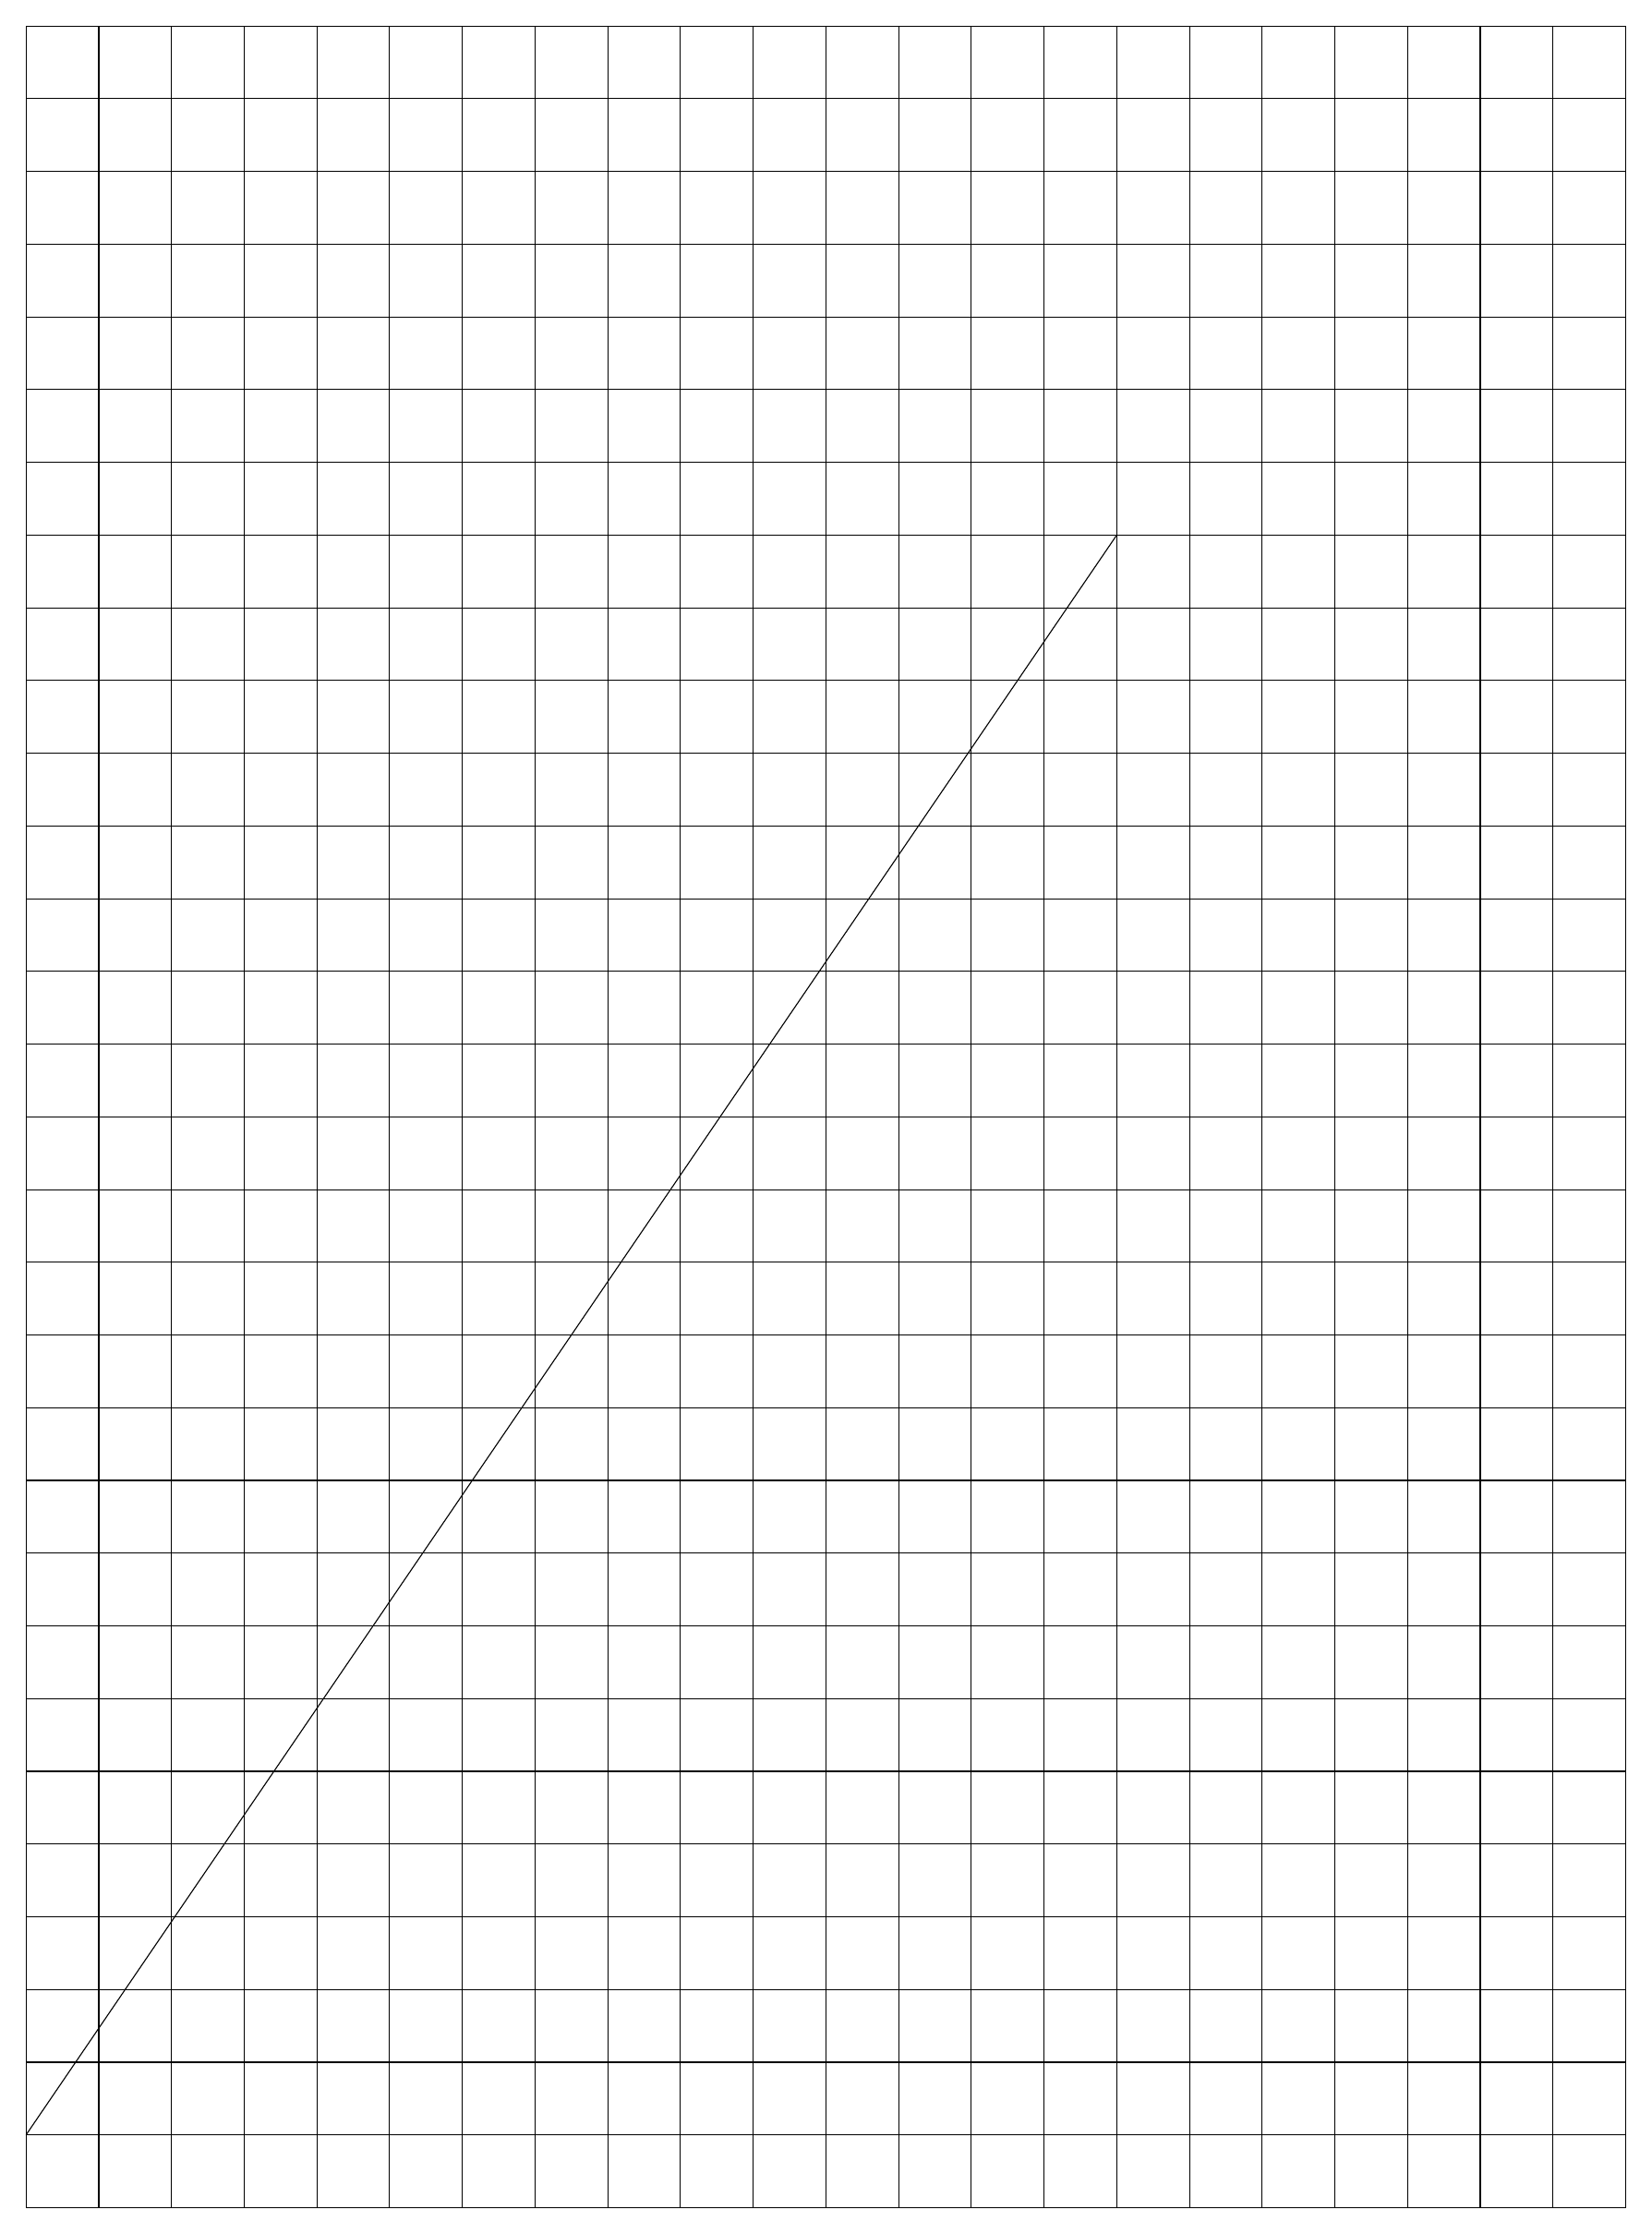
\begin{tikzpicture}
	% Grid
	\draw[](0,-3) grid (22,27);

	% Example Line
	\draw(0,-2) -- (15,20);
\end{tikzpicture}
	
	% TITLE PAGE
	\newpage
	\restoregeometry		% Restore the default margins
	\maketitle				% Create title
	\thispagestyle{empty}	% Remove footnotes and headers
	\vfill					% Push remaining text to the bottom of the page
	\begin{center}
		Made with \LaTeX
	\end{center}
	%Test \parencites{HowHashPassword}
	
	\newpage
\tableofcontents
\newpage
\listoffigures
\newpage
\listoftables
\newpage
\lstlistoflistings	
	
	
	% NEXT PAGES
	\newpage
		
	\directlua{tex.print("Lua says: Hello World!")}
\section{Formatting Text Examples}
\begin{tcolorbox}[]
Testing a colour box
\end{tcolorbox}

\begin{tcolorbox}[colback=red!5!white, colframe=red!50!black,
	title=Fancy Colour Box]
	\gls{ex} of testing another colour box\\
	\gls{ex}
\end{tcolorbox}

This is a reference \parencites{SpaceSnifferFeatures}

\section{Lorem Ipsum}

\lipsum[1-3]
	
	\newpage


\begin{lstlisting}[language=Rust, style=test]
	// Your Rust code here
	fn main() {
		// Declare a mutable variable
		let mut x = 5; 
		
		// Print the initial value
		println!("The value of x is: {}", x); 
		
		// Change the value of x
		x = 6; 
		
		// Print the new value
		println!("The value of x is: {}", x); 
	}
\end{lstlisting}
	
	% BIBLIOGRAPHY
	\newpage
	\printbibliography
\end{document}